\begin{frame}[fragile]{Égalité physique : pile de Treiber}
\large
\begin{minted}{ocaml}
type 'a t =
  'a list Atomic.t

let create () =
  Atomic.make []

let rec push t v =
  let old = Atomic.get t in
  let new_ = v :: old in
  if not @@ Atomic.compare_and_set t old new_ then (
    Domain.cpu_relax () ;
    push t v
  )
\end{minted}
\end{frame}

\begin{frame}[fragile]{Partage}
\Large
\begin{minted}{ocaml}
let test1 = Some 0 == Some 0 (* true *)
let test2 = [0;1]  == [0;1]  (* true *)
\end{minted}
\end{frame}

\begin{frame}[fragile]{Conflits de représentation des valeurs}
\Large
\begin{minted}{ocaml}
let test1 = Obj.repr false == Obj.repr 0 (* true *)
let test2 = Obj.repr None  == Obj.repr 0 (* true *)
let test3 = Obj.repr []    == Obj.repr 0 (* true *)
\end{minted}
\end{frame}

\begin{frame}[fragile]{Partage + conflits}
\Large
\begin{minted}{ocaml}
type any =
  Any : 'a -> any

let test1 = Any false == Any 0 (* true *)
let test2 = Any None  == Any 0 (* true *)
let test3 = Any []    == Any 0 (* true *)
\end{minted}
\end{frame}

\begin{frame}[fragile]{Pile de Treiber}
\Large
\begin{minted}{ocaml}
let rec push t v =
  let old = Atomic.get t in
  let new_ = v :: old in
  if not @@ Atomic.compare_and_set t old new_ then (
    Domain.cpu_relax () ;
    push t v
  )
\end{minted}
\end{frame}

\begin{frame}[fragile]{Égalité physique : \texttt{Eio.Rcfd}}
\begin{minted}{ocaml}
type state = Open of Unix.file_descr | Closing of (unit -> unit)
type t = { mutable ops: int [@atomic]; mutable state: state [@atomic] }

let make fd = { ops= 0; state= Open fd }

let closed = Closing (fun () -> ())
let close t =
  match t.state with
  | Closing _ -> false
  | Open fd as prev ->
      let close () = Unix.close fd in
      let next = Closing close in
      if Atomic.Loc.compare_and_set [%atomic.loc t.state] prev next then
        ...
      else
        false
\end{minted}
\end{frame}

\begin{frame}[fragile]{Départage}
\Large
\begin{minted}{ocaml}
let x = Some 0
let test = x == x (* false *)
\end{minted}
\vfill
\begin{figure}
  \captionsetup{justification=centering}
  \begin{subfigure}[b]{0.3\textwidth}
    \centering
    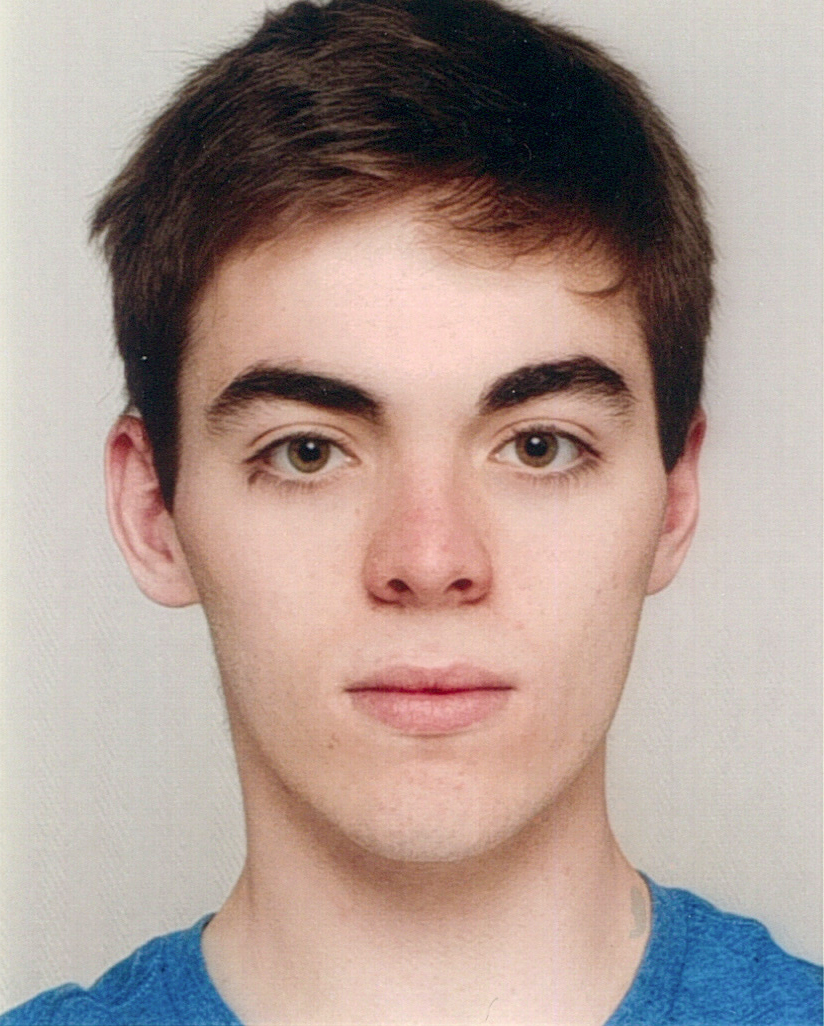
\includegraphics[height=3cm]{images/clement_allain.jpg}
    \caption*{\footnotesize \textbf{Clément Allain} \\ Impossible ! Identité unique.}
  \end{subfigure}
  \begin{subfigure}[b]{0.3\textwidth}
    \centering
    
\includegraphics[height=3cm]{images/armael_gueneau.jpg}
    \caption*{\footnotesize \textbf{Armaël Guéneau} \\ Ce serait du départage.}
  \end{subfigure}
  \begin{subfigure}[b]{0.3\textwidth}
    \centering
    
\includegraphics[height=3cm]{images/vincent_laviron.jpg}
    \caption*{\footnotesize \textbf{Vincent Laviron} \\ C'est possible !}
  \end{subfigure}
\end{figure}
\end{frame}

\begin{frame}[fragile]{\texttt{Eio.Rcfd}}
\begin{minted}{ocaml}
let closed = Closing (fun () -> ())
let close t =
  match t.state with
  | Closing _ -> false
  | Open fd as prev ->
      let close () = Unix.close fd in
      let next = Closing close in
      if Atomic.Loc.compare_and_set [%atomic.loc t.state] prev next then
        ...
      else
        false
\end{minted}
\end{frame}

\begin{frame}[fragile]{Constructeurs génératifs}
\Large
\begin{minted}{ocaml}
type 'a liste =
  | Nil
  | Cons of 'a * 'a liste [@generative]

type state =
  | Open of Unix.file_descr [@generative] [@zoo.reveal]
  | Closing of (unit -> unit)
\end{minted}
\end{frame}
